\documentclass[12pt]{article}
\usepackage[paper=letterpaper, margin=0.8in]{geometry}

%% The graphicx package provides the includegraphics command.
\usepackage{graphicx}
%% The amssymb package provides various useful mathematical symbols
\usepackage{amssymb}
%% The amsthm package provides extended theorem environments
%% \usepackage{amsthm}
%% fix strange gensymb error
\usepackage{textcomp}
%% symbols, especially degree
\usepackage{gensymb}
%% scientific units
\usepackage{siunitx}
%% line spacing
\usepackage{setspace}
\doublespacing
%% put figures at the end
%\usepackage[nomarkers]{endfloat}
%% allow hyperlinks
%\usepackage{hyperref}
%% color comments
\usepackage{soul}
\usepackage{color}
%% left justification in tables
\usepackage{array}
\newcolumntype{P}[1]{>{\raggedright\arraybackslash}p{#1}}
%%references
\usepackage[round]{natbib}
%%landscape orientation
\usepackage{pdflscape}

\begin{document}

{\Large
\textbf\newline{Carry-over effects of larval microclimate on the transmission potential of a mosquito-borne pathogen}}

\bigskip

Michelle V. Evans,
Justine C. Shiau,
Nicole Solano,
Melinda A. Brindley,
John M. Drake,
Courtney C. Murdock
\smallskip

{\Large{Supplemental Figure Captions}}

\begin{figure}[h]
\centering
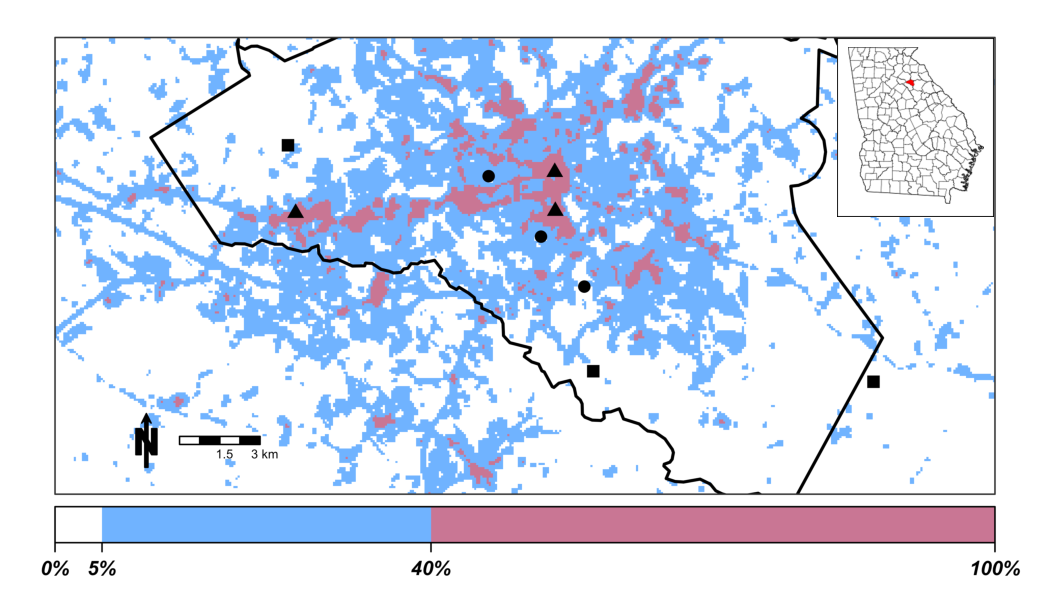
\includegraphics[width=6in]{SuppFig1.pdf}
\caption{\textbf{Supplemental Figure 1.} Map of study sites in Athens, GA, with inset illustrating location of Athens-Clarke County (black outline) in the state of Georgia. Symbols represent land classes (square: rural, circle:suburban, triangle: urban). Colors represent the amount of impervious surface within the 210m focal area of each pixel, as illustrated on the color bar on the bottom.}
\end{figure}

\begin{figure}
\centering
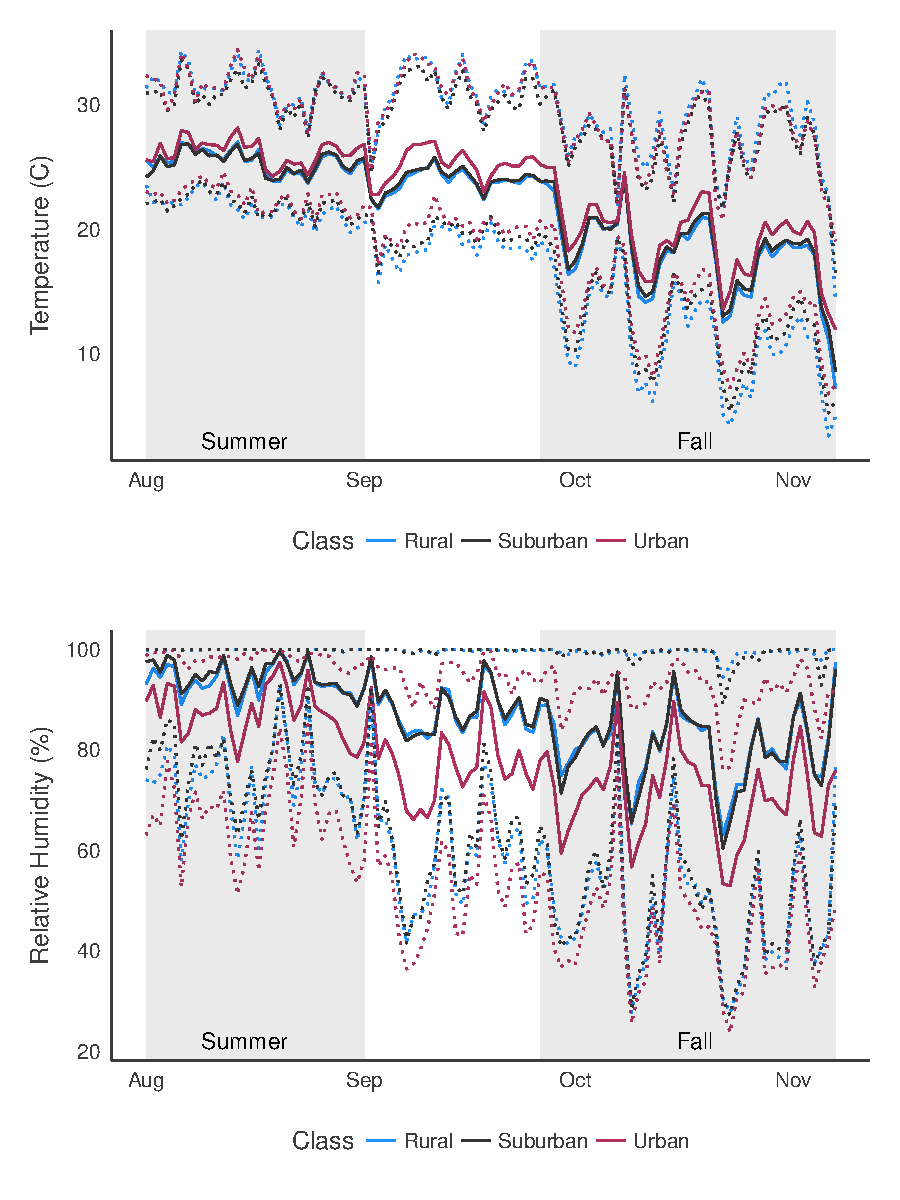
\includegraphics[width=6in]{SuppFig2.pdf}
\caption{\textbf{Supplemental Figure 2.} Microclimate differed significantly across both season and land class. The solid line represents the mean temperature and relative humidity across trays in each land class. The dotted lines represent the mean minimum and maximum temperature and relative humidity across trays in each land class.}
\end{figure}

\begin{figure}
\centering
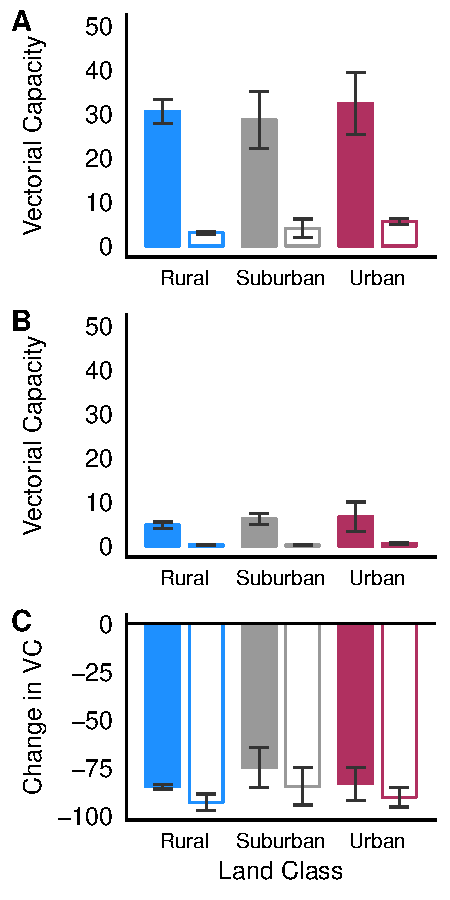
\includegraphics[width=3in]{SuppFig3.pdf}
\caption{\textbf{Supplemental Figure 3.} The incorporation of carry-over effects reduces the expected vectorial capacity at sites, although the effect is lessened in the fall. plots indicate calculated vectorial capacity without carry-over effects (a), with carry-over effects (b), and the percent difference due to the incorporation of carry-over effects (c). Error bars represent standard error.}
\end{figure}



\newpage

\end{document}
